%%%%%%%%%%%%%%%%%%%%%%%%%%%%%%%%%%%%%%%%%
% Presentation Template
% LaTeX Template
% Version 2.2 (2023-07-17)
%
% This template was adapted by:
% Jonathan Decker (jonathan.decker@uni-goettingen.de)
% From a template made by:
% Julian Kunkel (julian.kunkel@gwdg.de)
%
%%%%%%%%%%%%%%%%%%%%%%%%%%%%%%%%%%%%%%%%%
\documentclass[compress,aspectratio=169]{beamer}

% make sure the theme and config files are on this path
\usepackage[GI]{assets/beamerConfig}

\addbibresource{ref.bib}
\graphicspath{{.}{assets/}}

% --- document configuration ---
\newcommand{\mytitle}{Introduction to Git}
% Leave empty for no subtitle
\newcommand{\mysubtitle}{How to share code and collaborate with others!}
\newcommand{\myauthor}{Lars Quentin}
\newcommand{\myauthorurl}{}
\newcommand{\myvenue}{INFORMATIK 2023}
% For example, use \today
\newcommand{\mydate}{27.09.2023}
% For example, Institute for Computer Science / GWDG
\newcommand{\myinstitute}{GWDG / Campus-Institut Data Science}

\configuretitlepage

\begin{document}

	\begin{frame}[plain]
		\titlepage
	\end{frame}

	\begin{frame}[t]{Table of contents}
		\tableofcontents[subsectionstyle=hide/hide]
	\end{frame}

	% --- slides begin ---

	\begin{frame}{Goals}
		\begin{itemize}
			\item TODO
		\end{itemize}
	\end{frame}

	\section{Motivation}

	\begin{frame}{Original Problem}
    \begin{block}{How did people work together on code before?}
		  \begin{itemize}
        \item Make sure they weren't interefering each other:
          \begin{enumerate}
            \item Sending updated source code archives
            \item Shared Directory and file locks
            \item Shared Directory and luck
          \end{enumerate}
		  	\item Code Backups were done manually
        \item Problems with that approach:
          \begin{itemize}
            \item If shared directory, they can overwrite it accidentally
            \item Local versons were vastly different, hard to merge together
            \item Everything relied on a lot of communication and manual work.
          \end{itemize}
		  \end{itemize}
    \end{block}
	\end{frame}

  \begin{frame}{Solution: Git}
    \begin{columns}
      \begin{column}{0.5\textwidth}
        \begin{itemize}
          \item Git is a \textbf{distributed version control system} (\textbf{VCS})
          \item Initially developed for the Linux kernel
          \item Bundles set of changes into named updates, called \textbf{commits}
          \item People can create their own updates, \textbf{branching} out
          \item Allows for huge collaboration
            \begin{itemize}
              \item Linux has over 1400 contributors! \cite{contrib}
            \end{itemize}
        \end{itemize}
      \end{column}
      \begin{column}{0.5\textwidth}
        \begin{figure}
          
\includegraphics[width=\textwidth]{./assets/Git.png}
          \caption{Git Logo \cite{git}}
        \end{figure}
      \end{column}
    \end{columns}
  \end{frame}

  \begin{frame}{Git is not GitHub}
    \begin{columns}
      \begin{column}{0.6\textwidth}
        \begin{itemize}
          \item Git is a program for versioning
          \item GitHub is a website that hosts Git projects
          \item Git is not made by Github
          \item Analogy: E-Mail
            \begin{itemize}
              \item Outlook (the program) is an Email-Client
              \item Google Mail is a Email hoster
              \item Outlook is not made by Google!
            \end{itemize}
        \end{itemize}
      \end{column}
      \begin{column}{0.4\textwidth}
        \begin{figure}
          
\includegraphics[width=0.5\textwidth]{./assets/GitHub.png}
          \caption{GitHub Logo \cite{ghlogo}}
        \end{figure}
        \begin{figure}
          
\includegraphics[width=0.6\textwidth]{./assets/octocat.png}
          \caption{GitHub Mascot: Octocat \cite{octodex}}
        \end{figure}
      \end{column}
    \end{columns}
  \end{frame}

  \begin{frame}{Why to use Git}
    \begin{itemize}
      \item Collaborate with others
      \item Manage multiple, actively worked on versions
        \begin{itemize}
          \item 2 people can't trivially write in the same file!
        \end{itemize}
      \item Version your code, take more risks, roll back mistakes!
      \item Make your code more discoverable
        \begin{itemize}
          \item It's common to Google: ``\texttt{<MY PROBLEM> github}''
          \item Better discoverability than personal website
        \end{itemize}
      \item Use Github/Gitlab as an portfolio
    \end{itemize}
  \end{frame}

	\section{Theory}

	\begin{frame}{How does Git work?}
		\begin{itemize}
      \item Git projects are called \textbf{repositories} or \textbf{repos}
      \item There are 2 ways to create a Git repository
        \begin{itemize}
          \item \textbf{Initialize} a new folder (Create)
          \item \textbf{Clone} an existing repo (Download)
        \end{itemize}
      \item This means that it is \textbf{local} on your device
        \begin{itemize}
          \item Just a normal folder you can work in with any tools!
        \end{itemize}
      \item Once you finished something, you can bundle it into an update
        \begin{itemize}
          \item A so-called \textbf{commit}
        \end{itemize}
		\end{itemize}
	\end{frame}

  \begin{frame}{What does \textbf{Distributed} mean?}
    \begin{columns}
      \begin{column}{0.5\textwidth}
        \begin{itemize}
          \item Once you \textbf{initialize} or \textbf{clone} the repo, it is local on the device.
            \begin{itemize}
              \item You do \emph{not} work on the remote server!
            \end{itemize}
          \item Every developer has its local version
            \begin{itemize}
              \item It doesn't change automatically!
            \end{itemize}
          \item Instead, one can manually
            \begin{itemize}
              \item \textbf{Pull} the newest commits from the server
              \item \textbf{Push} the local commits to the server
            \end{itemize}
        \end{itemize}
      \end{column}
      \begin{column}{0.5\textwidth}
        \begin{figure}
          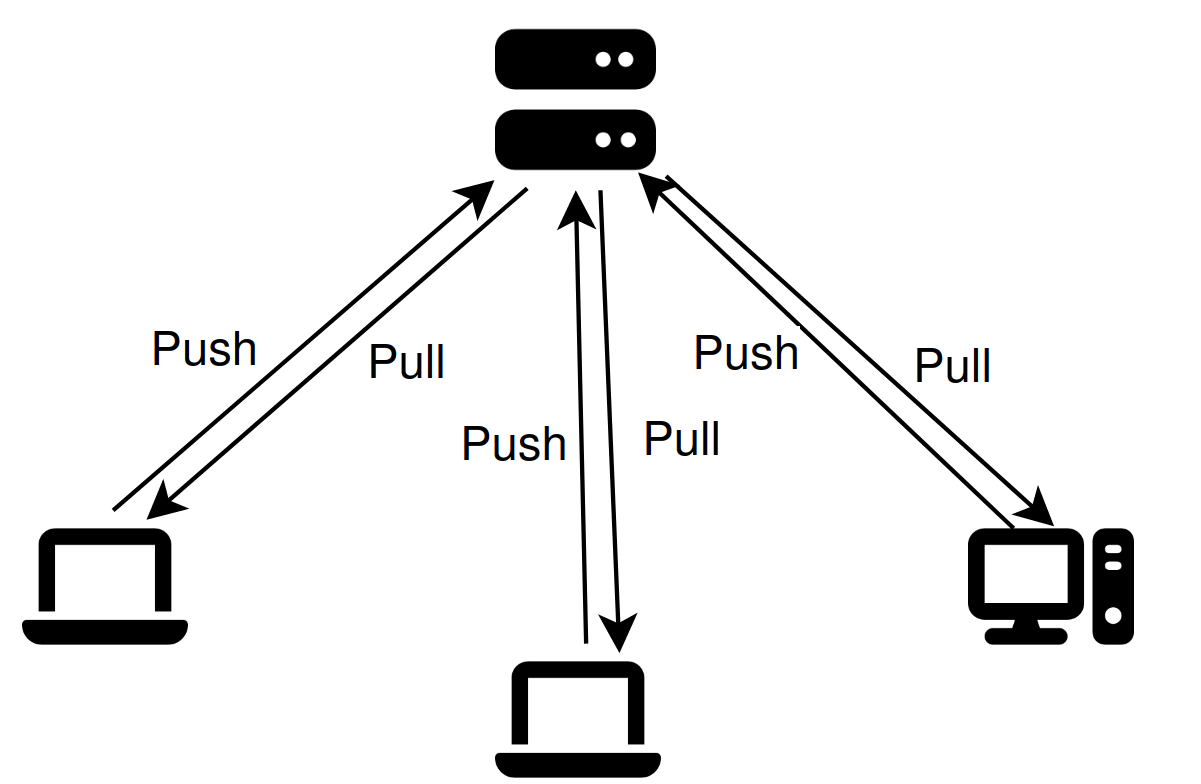
\includegraphics[width=\textwidth]{./assets/dist.png}
          \caption{Every computer has a local version.}
        \end{figure}
      \end{column}
    \end{columns}
  \end{frame}

  \begin{frame}{About Commits}
    \begin{columns}
      \begin{column}{0.6\textwidth}
        \begin{block}{Git is (mainly) for text files!}
          \begin{itemize}
            \item Because it tracks changes line by line
            \item The following are \textbf{NOT} text files:
              \begin{itemize}
                \item Word files (\texttt{.docx})
                \item PDFs
                \item Audio, Video, Pictures...
              \end{itemize}
            \item Non text files can be put into git
              \begin{itemize}
                \item Fullly replaced everytime!
              \end{itemize}
            \item A commit is the \textbf{difference} in lines
              \begin{itemize}
                \item Called a \textbf{diff}
              \end{itemize}
          \end{itemize}
        \end{block}
      \end{column}
      \begin{column}{0.4\textwidth}
        \begin{figure}
          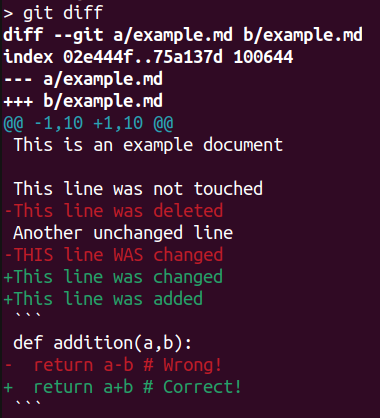
\includegraphics[width=0.9\textwidth]{./assets/diff.png}
          \caption{Red is deleted, green is added}
        \end{figure}
      \end{column}
    \end{columns}
  \end{frame}

  \begin{frame}{About Commits (cont.)}
    \begin{block}{When should you commit}
      \begin{itemize}
        \item If you can describe what you have done.
          \begin{itemize}
            \item Think of an experiment log.
            \item "I am currently filling the 41st ml into this flask!"
          \end{itemize}
        \item Why do we commit:
          \begin{itemize}
            \item Better understanding for others
            \item Better understanding for our future self
          \end{itemize}
      \end{itemize}
    \end{block}
  \end{frame}

	\section{Getting Started}

	\begin{frame}{Installing Git}
    \begin{figure}
      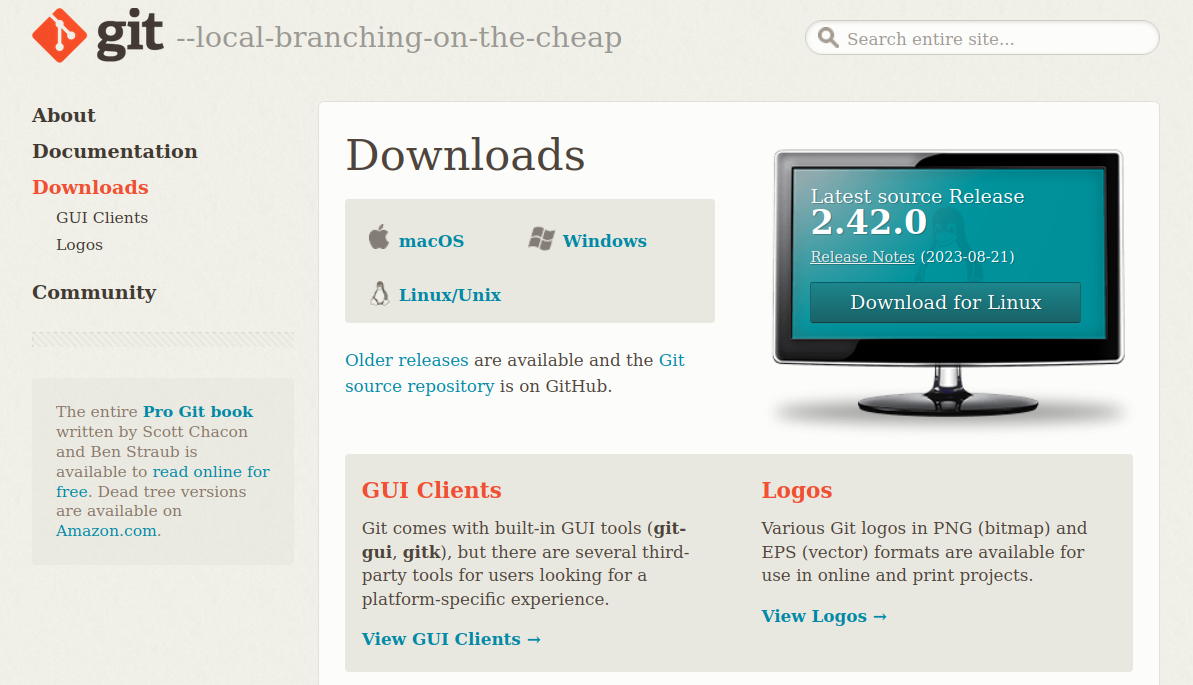
\includegraphics[width=0.8\textwidth]{./assets/gitwebsite.png}
    \end{figure}
	\end{frame}

  \begin{frame}{Initial configuration}
    Before starting, we have to do the following:
    \begin{itemize}
      \item Check whether it is installed
      \item Configure an SSH key
      \item Set an author and Email adress
    \end{itemize}
    \begin{center}
    \Large All on the exercises!
    \end{center}
  \end{frame}

  \begin{frame}{Create Repository (GitHub)}
    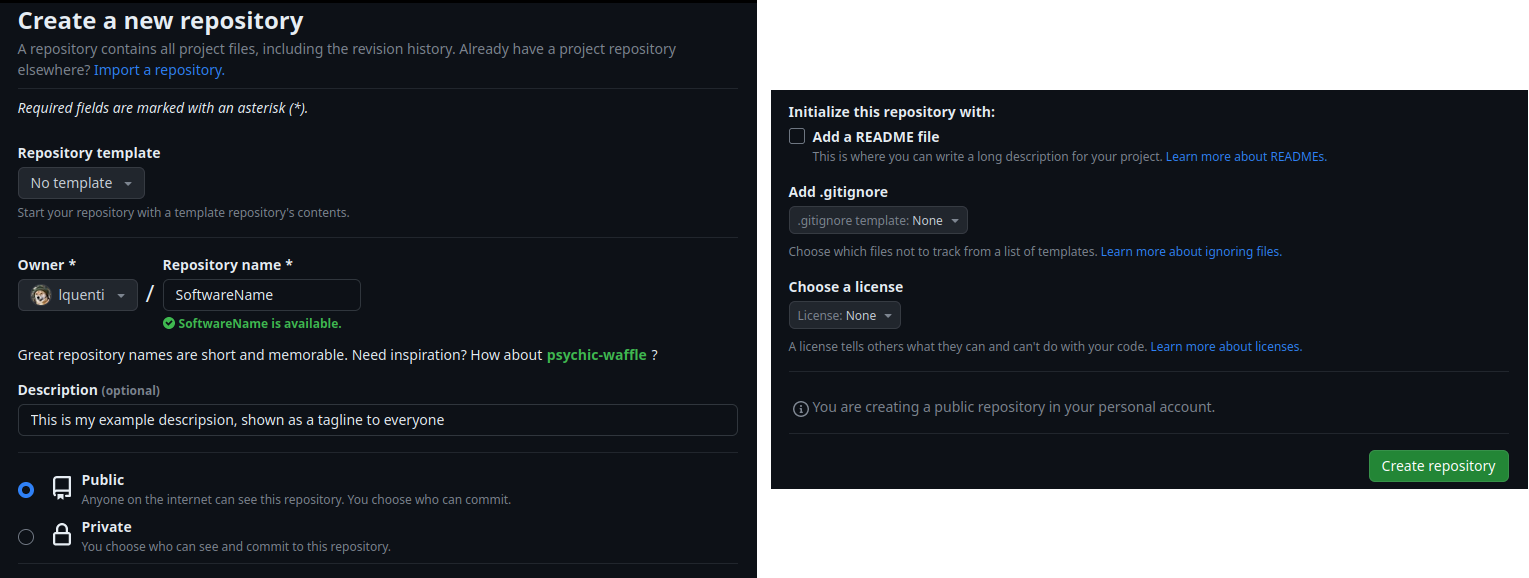
\includegraphics[width=\textwidth]{./assets/gh.png}
    \begin{center}
      Link: \href{https://github.com/new}{\url{https://github.com/new}}
    \end{center}
  \end{frame}

  % GIMP project in assets...
  \begin{frame}{Starting a local repository}
    
\includegraphics[width=\textwidth]{./assets/terminal_slideshows/01_add_existing_repo_01.png}
  \end{frame}
  \begin{frame}[noframenumbering]{Starting a local repository}
    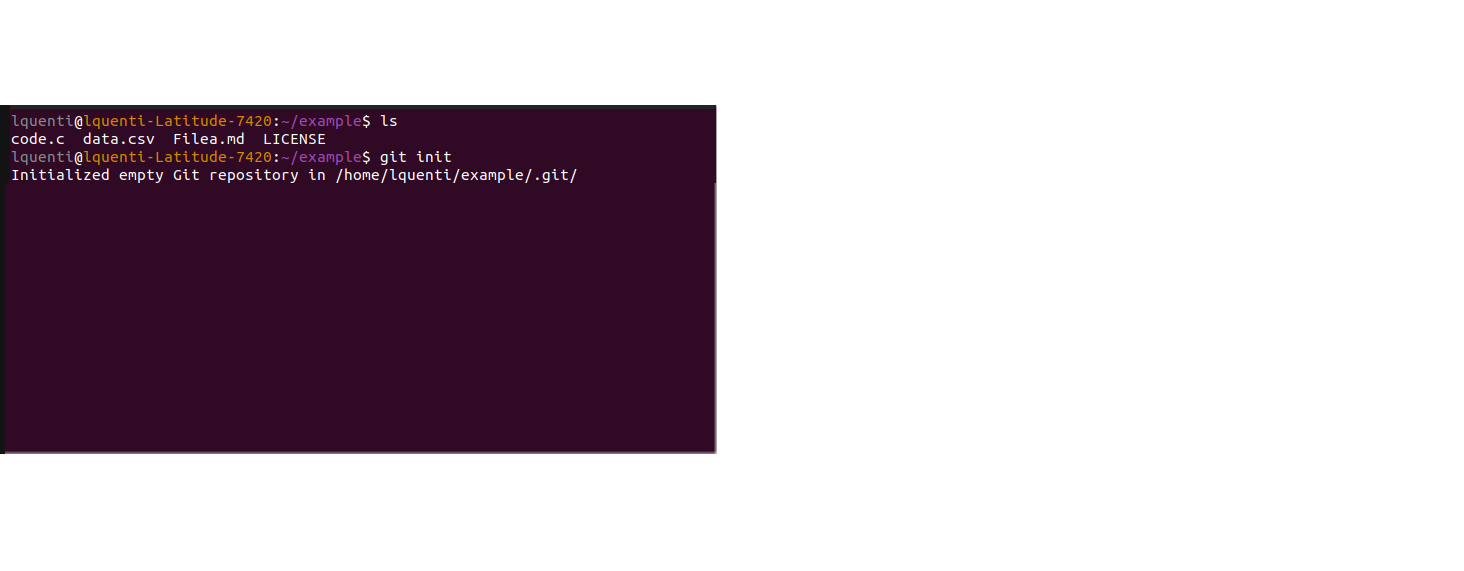
\includegraphics[width=\textwidth]{./assets/terminal_slideshows/01_add_existing_repo_02.png}
  \end{frame}
  \begin{frame}[noframenumbering]{Starting a local repository}
    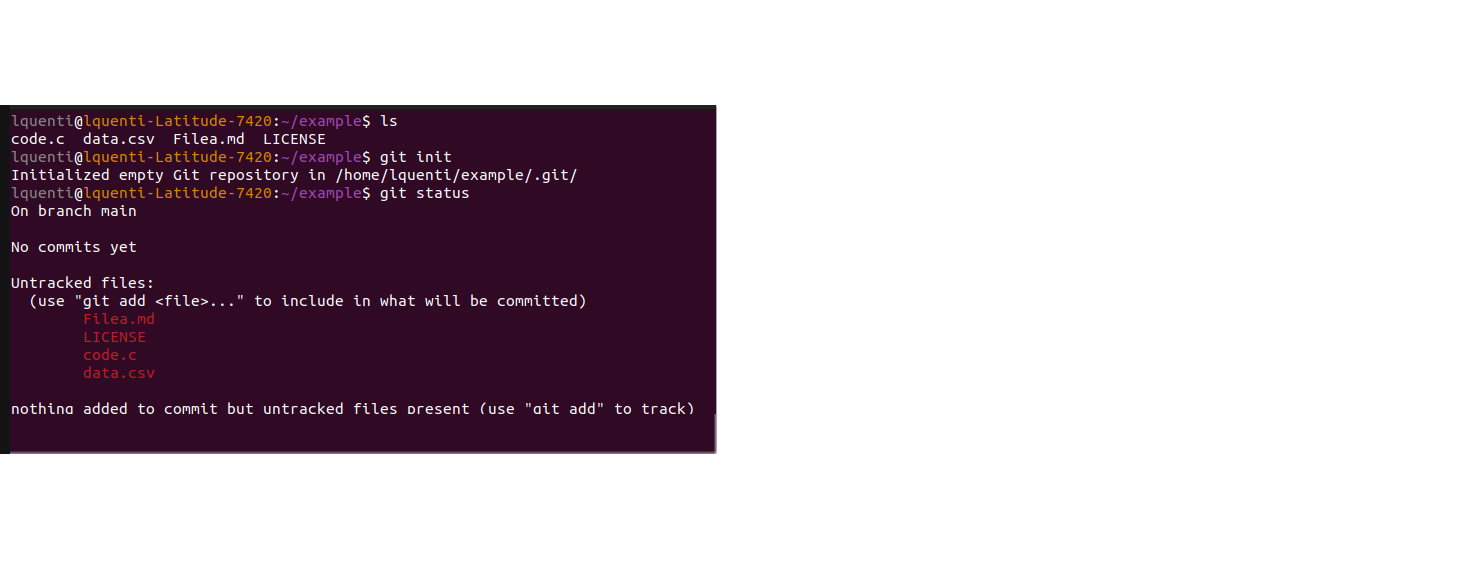
\includegraphics[width=\textwidth]{./assets/terminal_slideshows/01_add_existing_repo_03.png}
  \end{frame}
  \begin{frame}[noframenumbering]{Starting a local repository}
    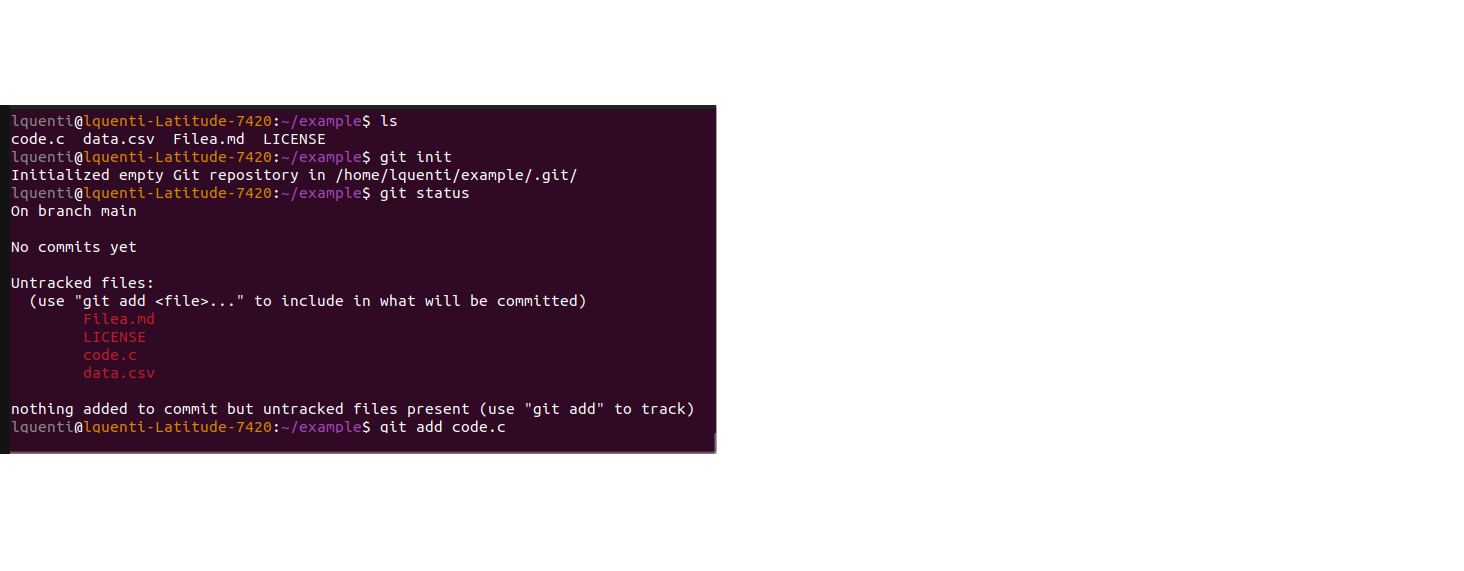
\includegraphics[width=\textwidth]{./assets/terminal_slideshows/01_add_existing_repo_04.png}
  \end{frame}
  \begin{frame}[noframenumbering]{Starting a local repository}
    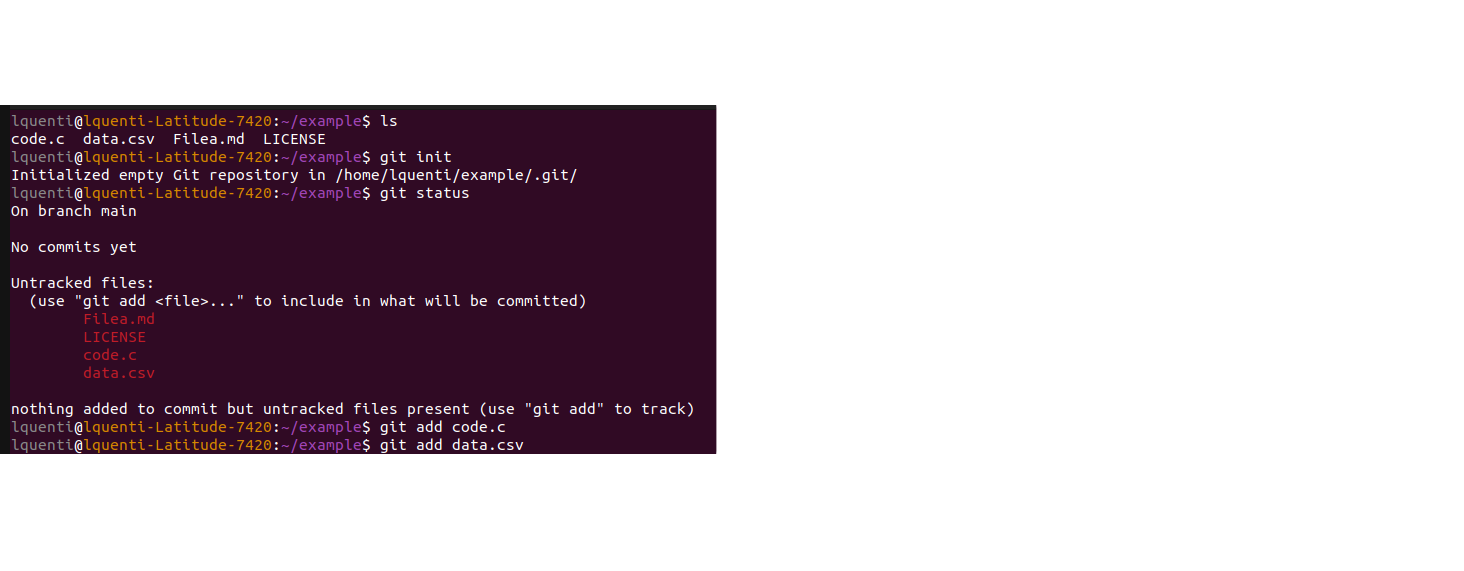
\includegraphics[width=\textwidth]{./assets/terminal_slideshows/01_add_existing_repo_05.png}
  \end{frame}
  \begin{frame}[noframenumbering]{Starting a local repository}
    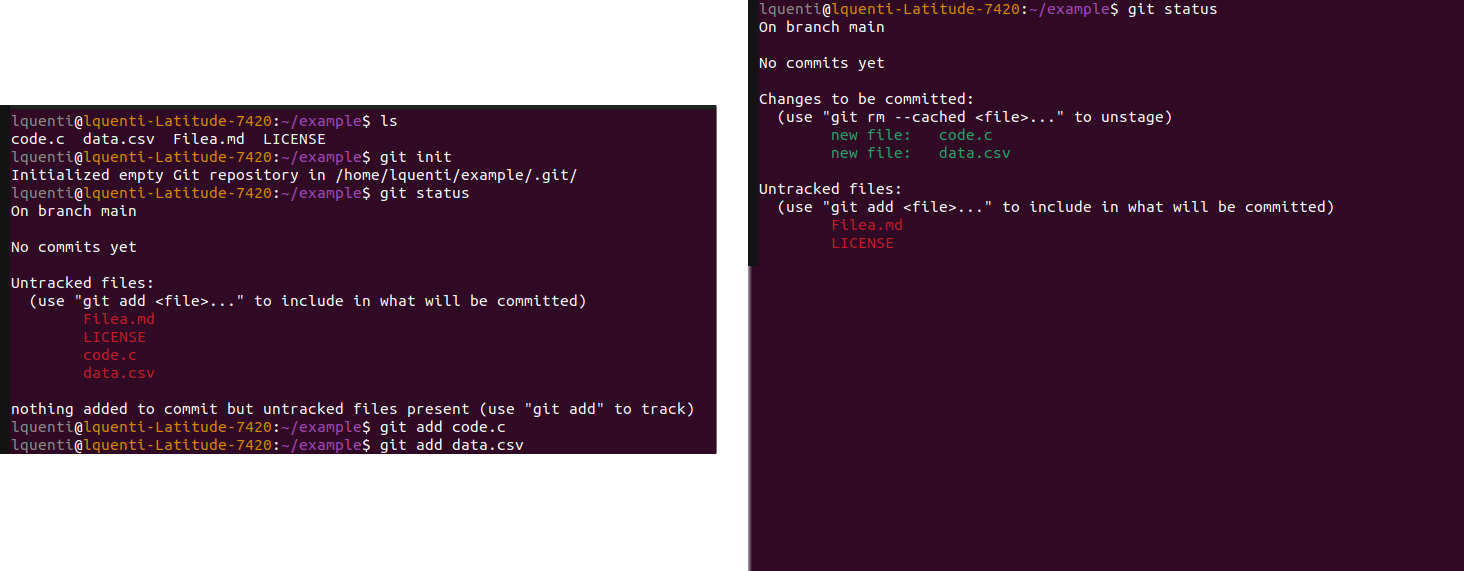
\includegraphics[width=\textwidth]{./assets/terminal_slideshows/01_add_existing_repo_06.png}
  \end{frame}
  \begin{frame}[noframenumbering]{Starting a local repository}
    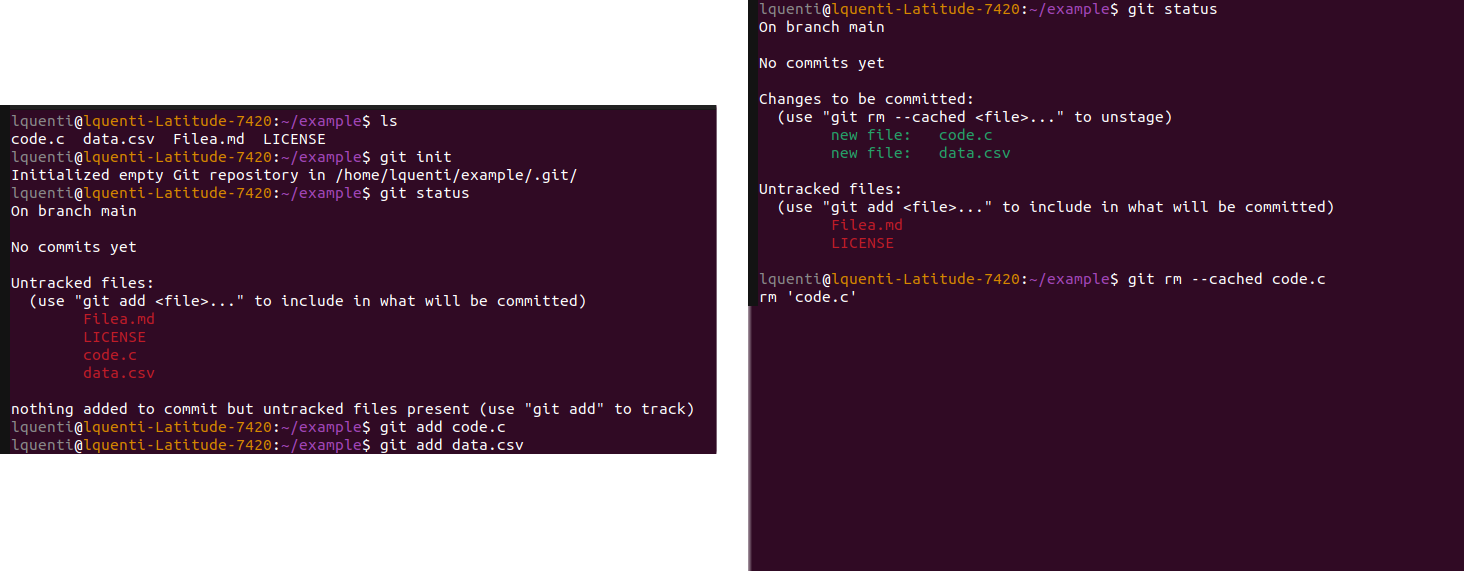
\includegraphics[width=\textwidth]{./assets/terminal_slideshows/01_add_existing_repo_07.png}
  \end{frame}
  \begin{frame}[noframenumbering]{Starting a local repository}
    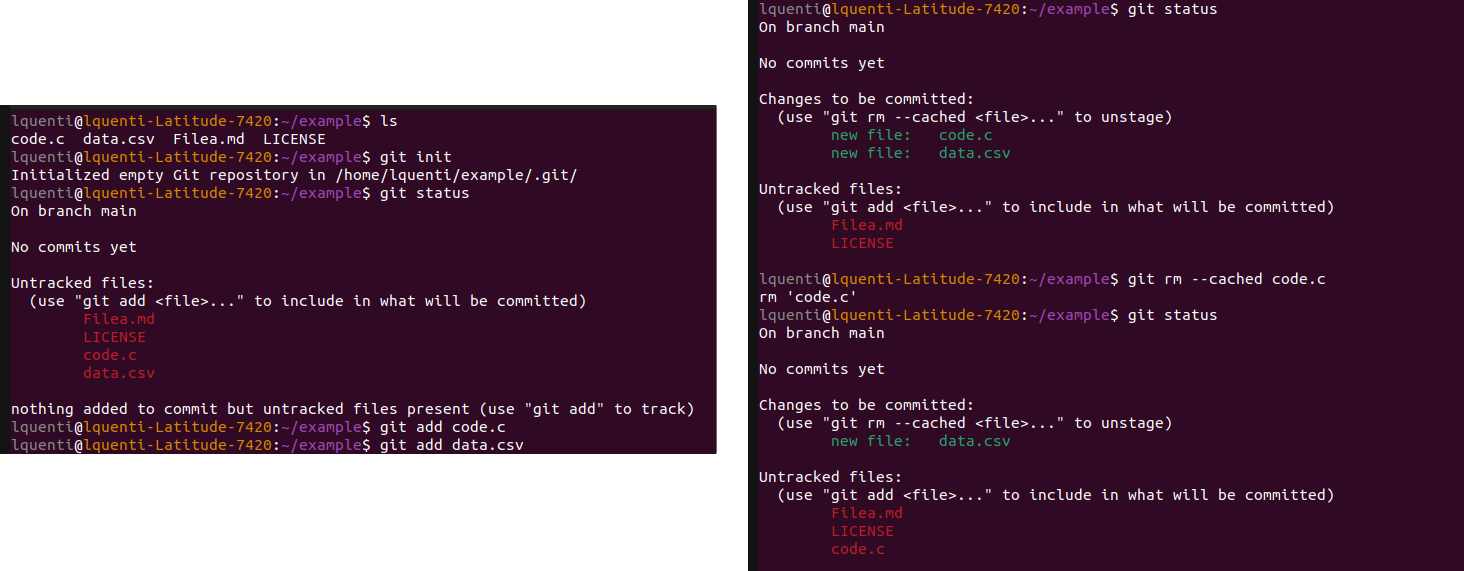
\includegraphics[width=\textwidth]{./assets/terminal_slideshows/01_add_existing_repo_08.png}
  \end{frame}

  \begin{frame}{Creating a commit}
    \begin{center}
      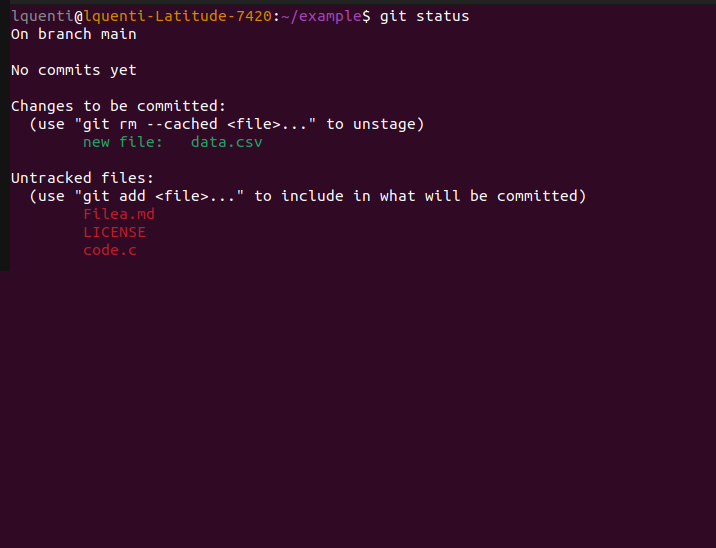
\includegraphics[height=0.85\textheight]{./assets/terminal_slideshows/02_commits_01.png}
    \end{center}
  \end{frame}
  \begin{frame}[noframenumbering]{Creating a commit}
    \begin{center}
      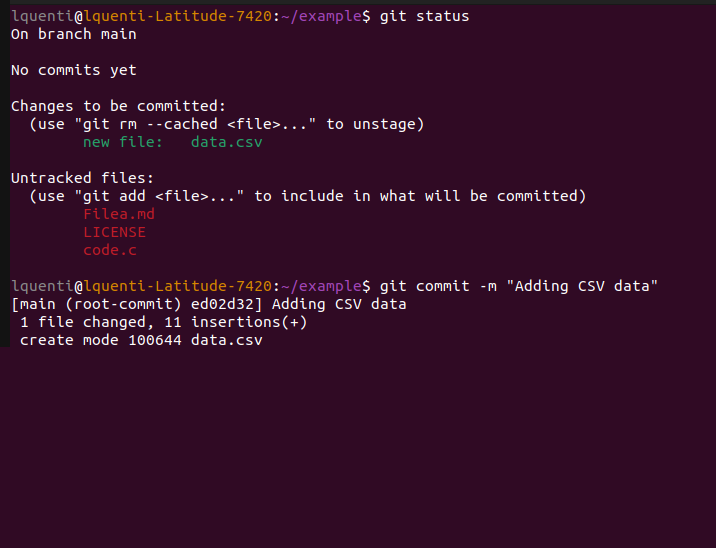
\includegraphics[height=0.85\textheight]{./assets/terminal_slideshows/02_commits_02.png}
    \end{center}
  \end{frame}
  \begin{frame}[noframenumbering]{Creating a commit}
    \begin{center}
      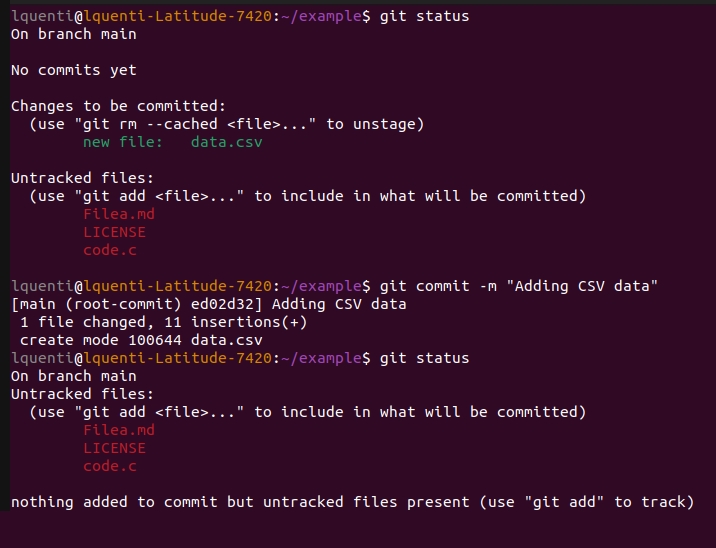
\includegraphics[height=0.85\textheight]{./assets/terminal_slideshows/02_commits_03.png}
    \end{center}
  \end{frame}
  \begin{frame}[noframenumbering]{Creating a commit}
    \begin{center}
      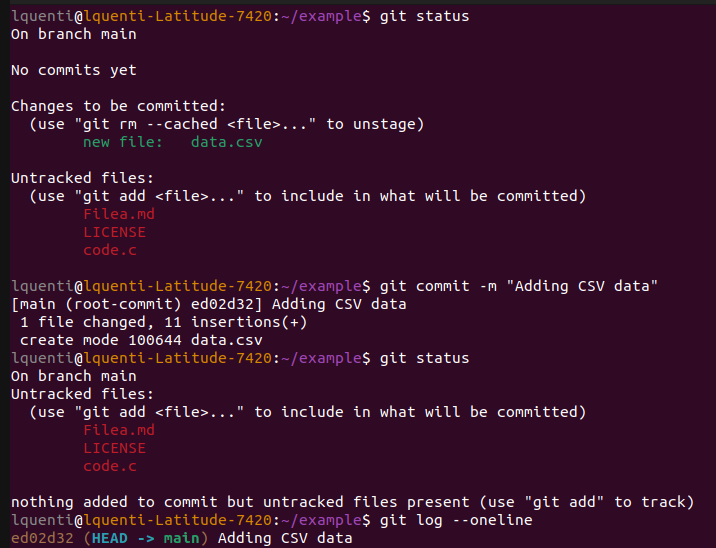
\includegraphics[height=0.85\textheight]{./assets/terminal_slideshows/02_commits_04.png}
    \end{center}
  \end{frame}

  \begin{frame}{Push and pull updates}
    \begin{center}
      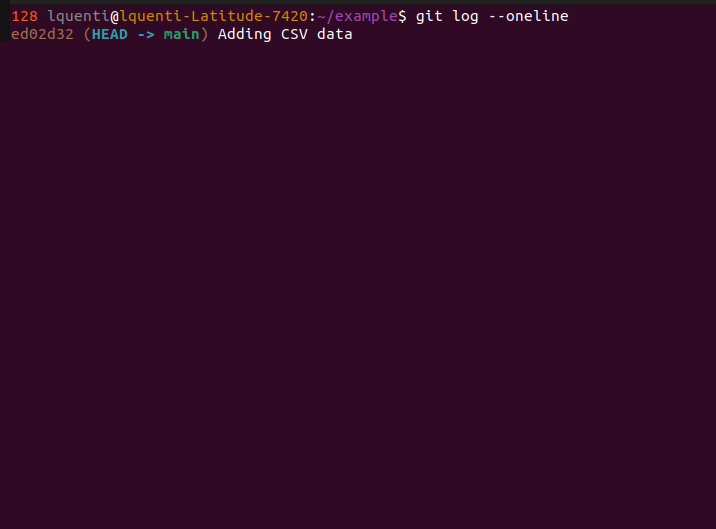
\includegraphics[height=0.85\textheight]{./assets/terminal_slideshows/03_Push_Pull_01.png}
    \end{center}
  \end{frame}
  \begin{frame}[noframenumbering]{Creating a commit}
    \begin{center}
      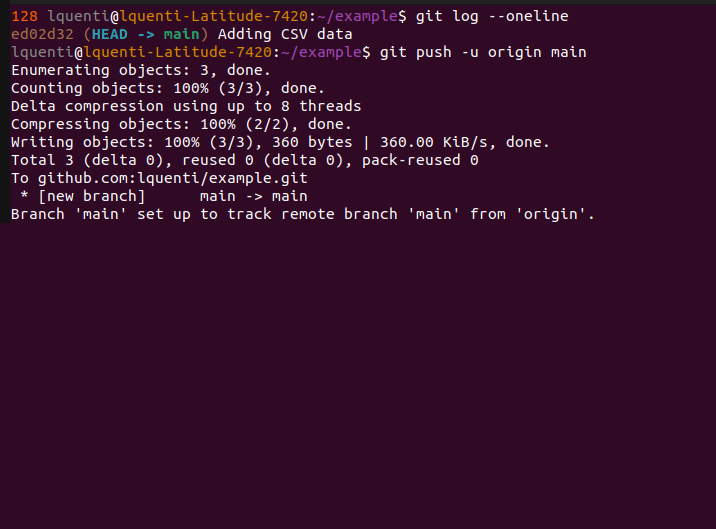
\includegraphics[height=0.85\textheight]{./assets/terminal_slideshows/03_Push_Pull_02.png}
    \end{center}
  \end{frame}
  \begin{frame}[noframenumbering]{Creating a commit}
    \begin{center}
      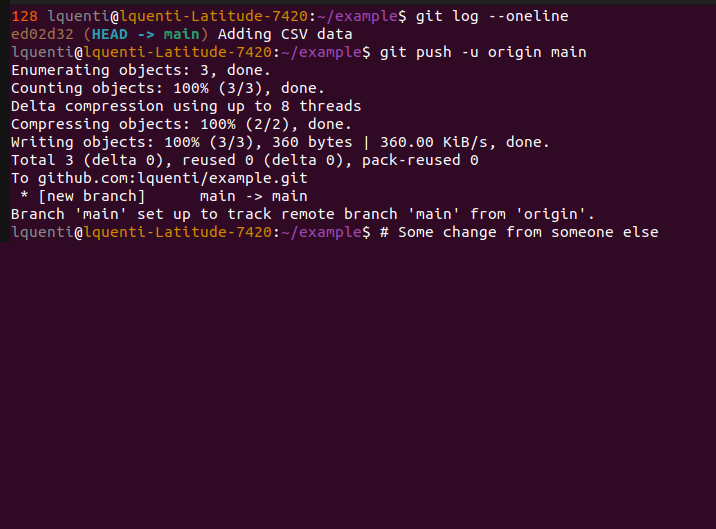
\includegraphics[height=0.85\textheight]{./assets/terminal_slideshows/03_Push_Pull_03.png}
    \end{center}
  \end{frame}
  \begin{frame}[noframenumbering]{Creating a commit}
    \begin{center}
      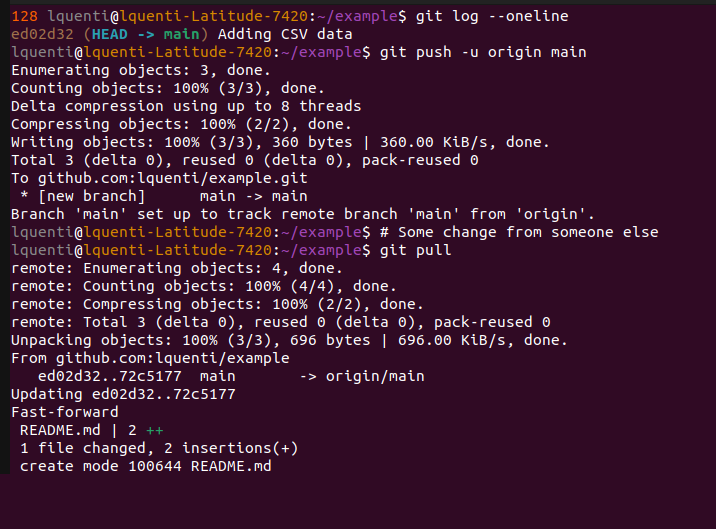
\includegraphics[height=0.85\textheight]{./assets/terminal_slideshows/03_Push_Pull_04.png}
    \end{center}
  \end{frame}
  \begin{frame}[noframenumbering]{Creating a commit}
    \begin{center}
      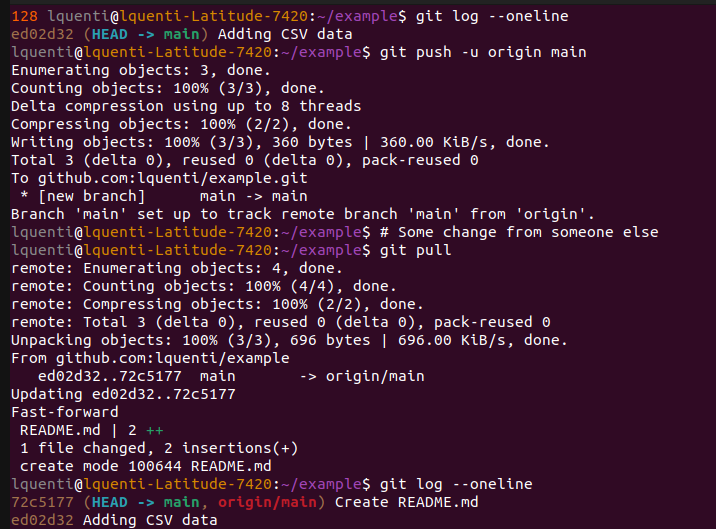
\includegraphics[height=0.85\textheight]{./assets/terminal_slideshows/03_Push_Pull_05.png}
    \end{center}
  \end{frame}

  \begin{frame}{Cloning a remote repository}
    \begin{center}
      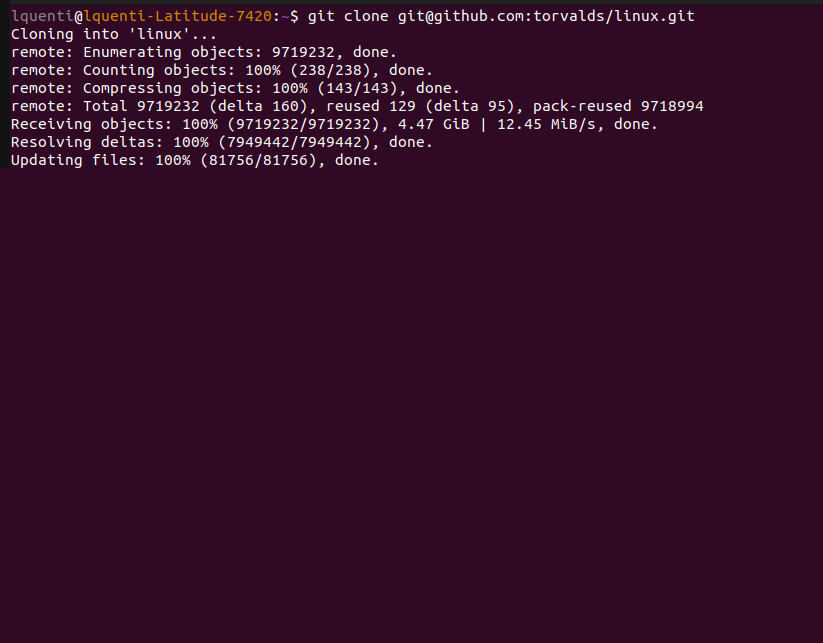
\includegraphics[height=0.85\textheight]{./assets/terminal_slideshows/04_clone_edit_01.png}
    \end{center}
  \end{frame}
  \begin{frame}[noframenumbering]{Cloning a remote repository}
    \begin{center}
      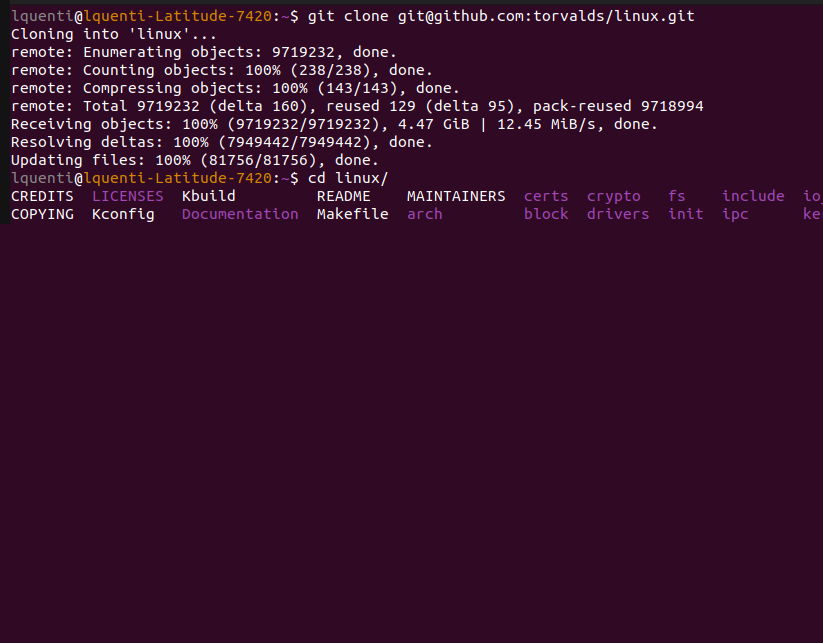
\includegraphics[height=0.85\textheight]{./assets/terminal_slideshows/04_clone_edit_02.png}
    \end{center}
  \end{frame}
  \begin{frame}[noframenumbering]{Cloning a remote repository}
    \begin{center}
      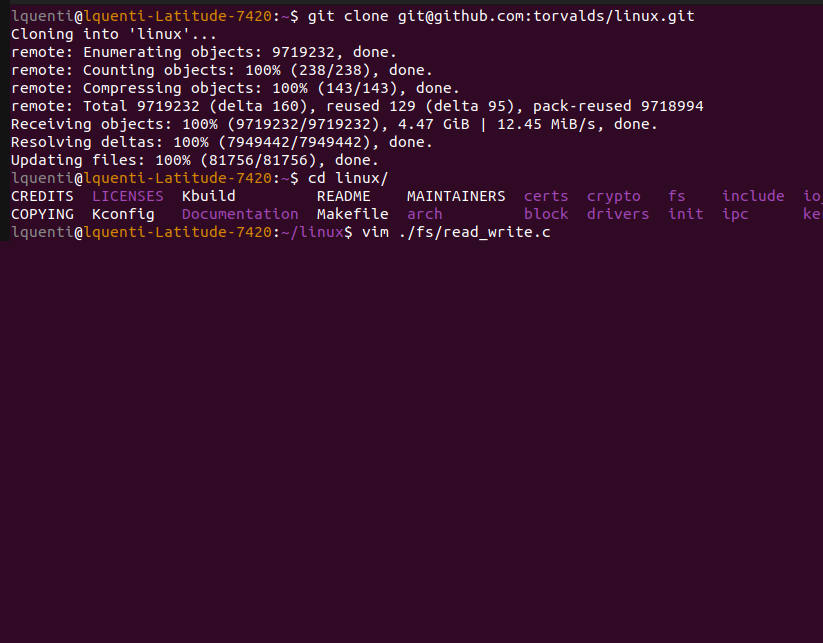
\includegraphics[height=0.85\textheight]{./assets/terminal_slideshows/04_clone_edit_03.png}
    \end{center}
  \end{frame}
  \begin{frame}[noframenumbering]{Cloning a remote repository}
    \begin{center}
      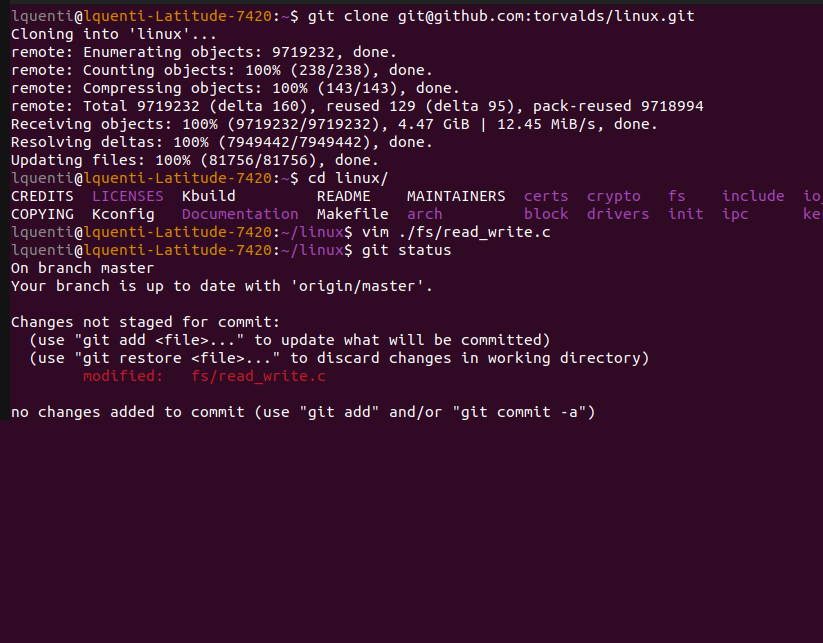
\includegraphics[height=0.85\textheight]{./assets/terminal_slideshows/04_clone_edit_04.png}
    \end{center}
  \end{frame}
  \begin{frame}[noframenumbering]{Cloning a remote repository}
    \begin{center}
      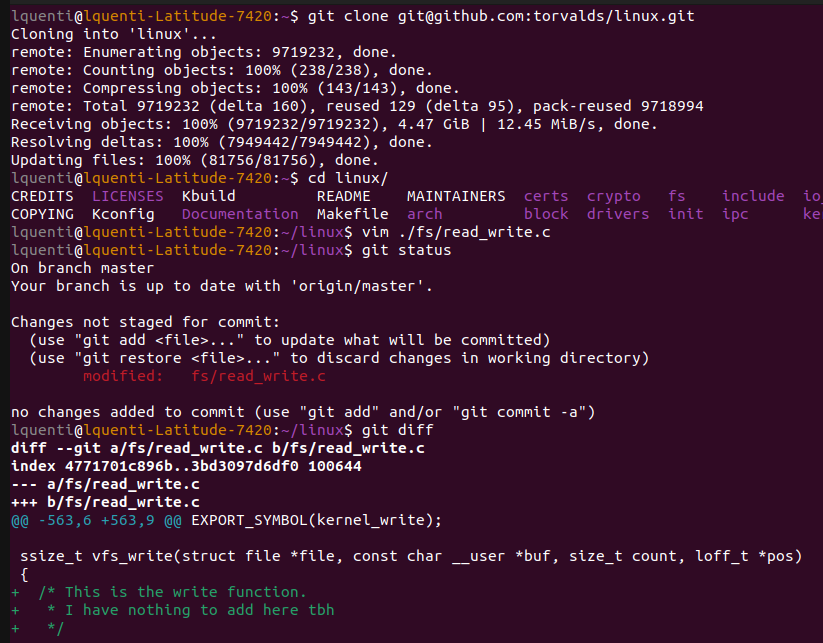
\includegraphics[height=0.85\textheight]{./assets/terminal_slideshows/04_clone_edit_05.png}
    \end{center}
  \end{frame}

  \section{GitHub GUI}

	\begin{frame}{Introduction to Git GUIs}
    \begin{columns}
      \begin{column}{0.5\textwidth}
        \begin{block}{Use a Git GUI?}
          \begin{itemize}
            \item Pro
              \begin{itemize}
                \item Flatter learning curve
                \item Visual representation
                \item Less memorization
              \end{itemize}
            \item Contra
              \begin{itemize}
                \item Less powerful
                \item Slower for advanced tasks
                \item Abstraction based vendor lock-in
              \end{itemize}
          \end{itemize}
          \begin{center}
            While it is worthwhile to learn git, a GUI can help initially!
          \end{center}
        \end{block}
      \end{column}
      \begin{column}{0.5\textwidth}
        \begin{block}{GitHub GUI}
          \begin{itemize}
            \item Supports many git features
            \item Only good ``multiplatform'' standalone GUI client
              \begin{itemize}
                \item Linux community-maintained
              \end{itemize}
            \item Supports Non-Git GitHub features
              \begin{itemize}
                \item Including CI/CD
              \end{itemize}
            \item Syntax Highlighted Diffs
            \item Git Branch visualization
          \end{itemize}
        \end{block}
      \end{column}
    \end{columns}
	\end{frame}

  \begin{frame}
    \begin{center}
      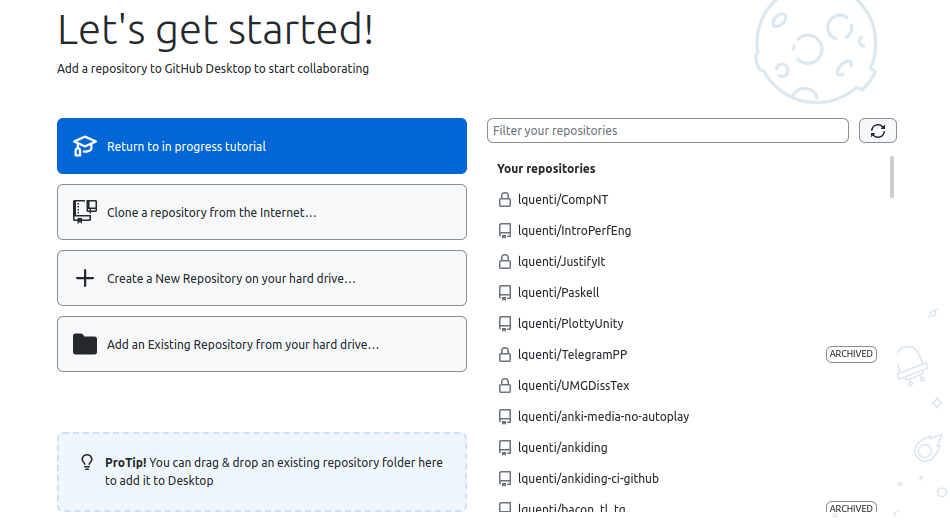
\includegraphics[height=0.85\textheight]{./assets/GHOverview.png}
    \end{center}
  \end{frame}

  \begin{frame}{In a repository}
    \begin{center}
      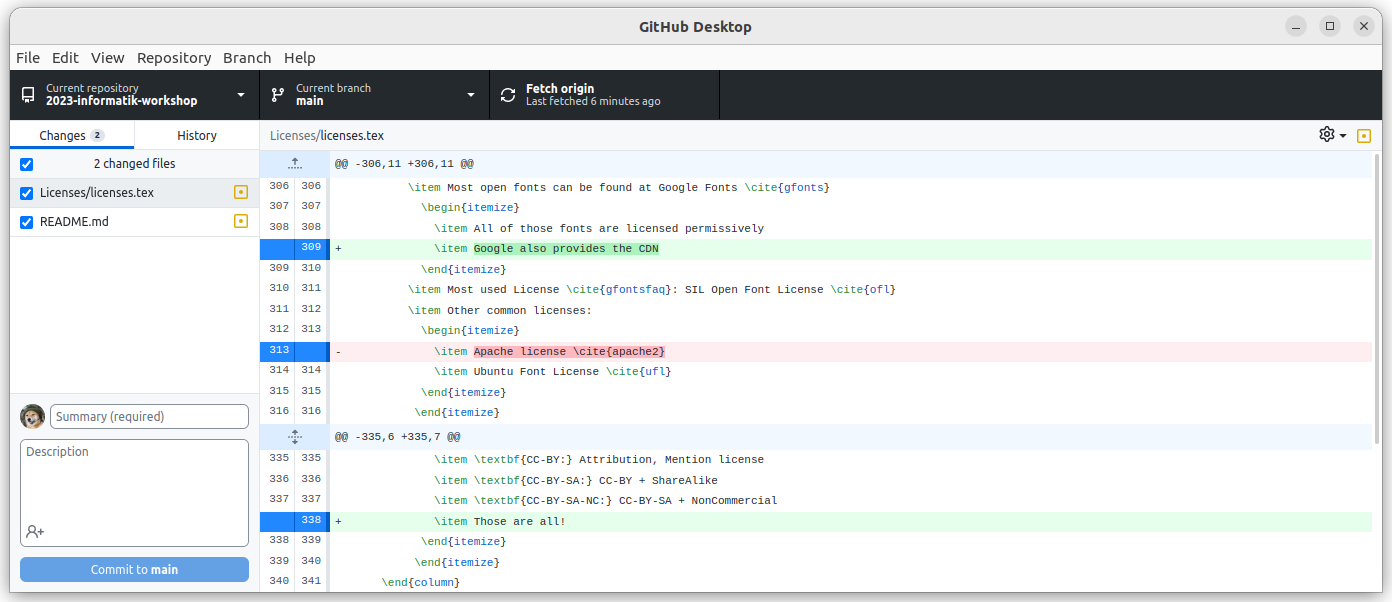
\includegraphics[height=0.75\textheight]{./assets/GH_01.png}
    \end{center}
  \end{frame}
  \begin{frame}[noframenumbering]{In a repository}
    \begin{center}
      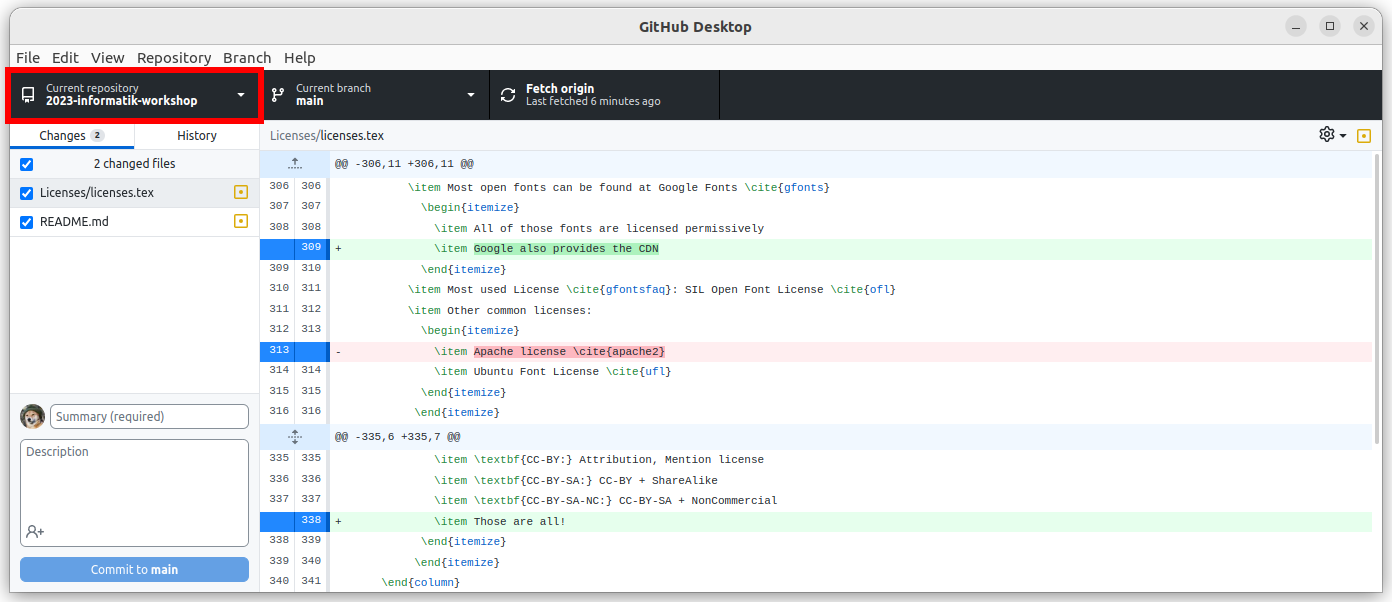
\includegraphics[height=0.75\textheight]{./assets/GH_01_01.png}
    \end{center}
  \end{frame}
  \begin{frame}[noframenumbering]{In a repository}
    \begin{center}
      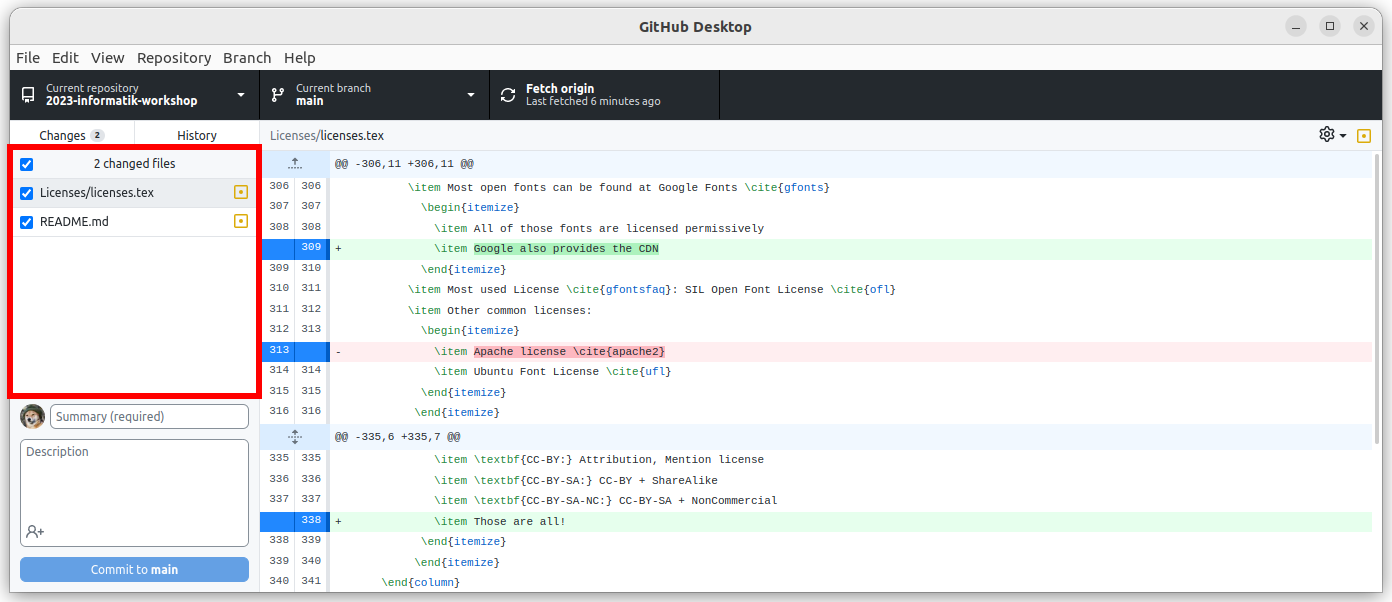
\includegraphics[height=0.75\textheight]{./assets/GH_01_02.png}
    \end{center}
  \end{frame}
  \begin{frame}[noframenumbering]{In a repository}
    \begin{center}
      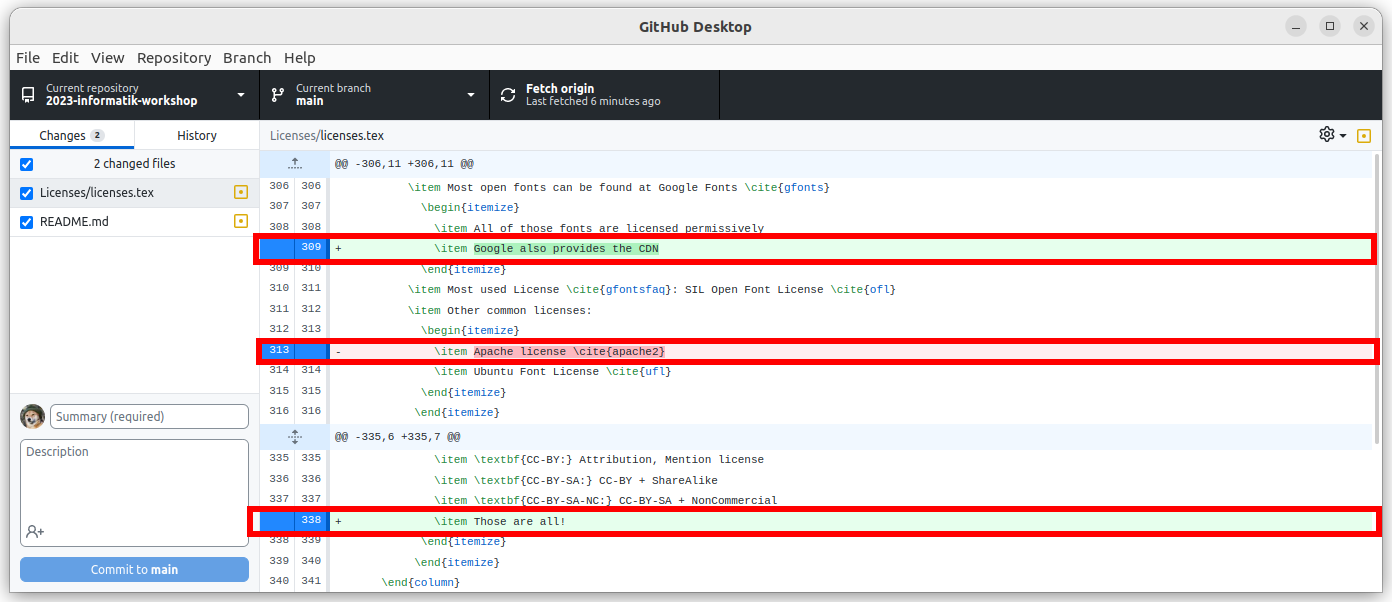
\includegraphics[height=0.75\textheight]{./assets/GH_01_03.png}
    \end{center}
  \end{frame}
  \begin{frame}[noframenumbering]{In a repository}
    \begin{center}
      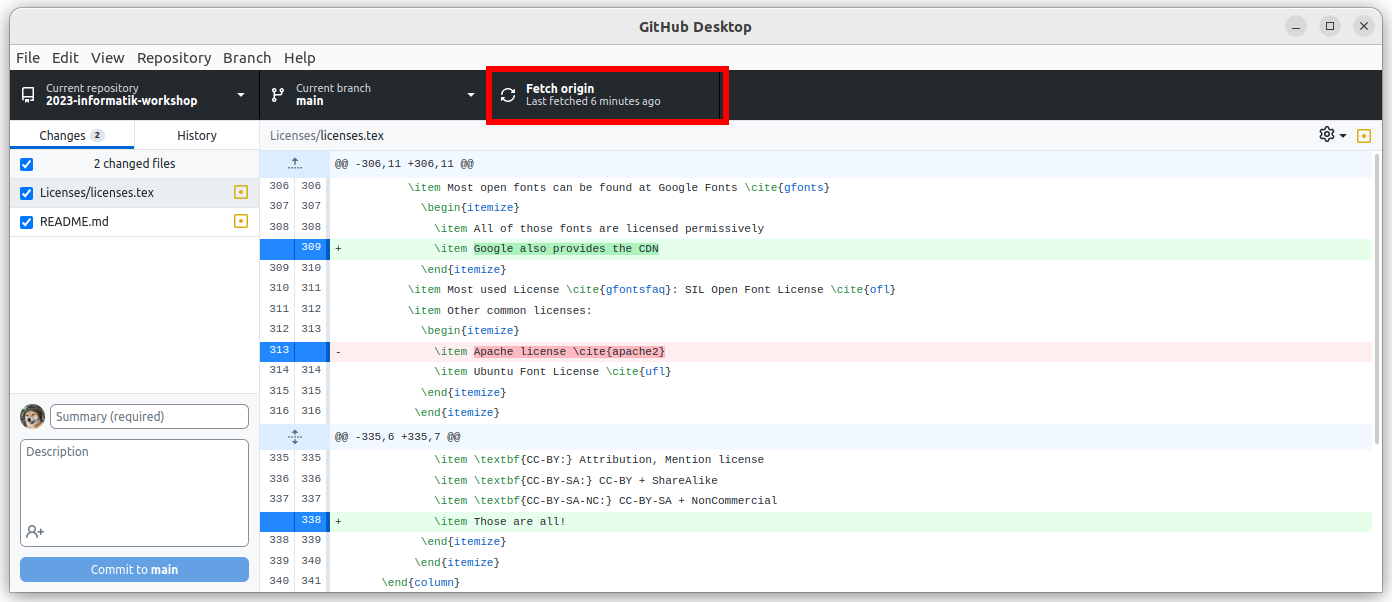
\includegraphics[height=0.75\textheight]{./assets/GH_01_04.png}
    \end{center}
  \end{frame}

  \begin{frame}{Committing}
    \begin{center}
      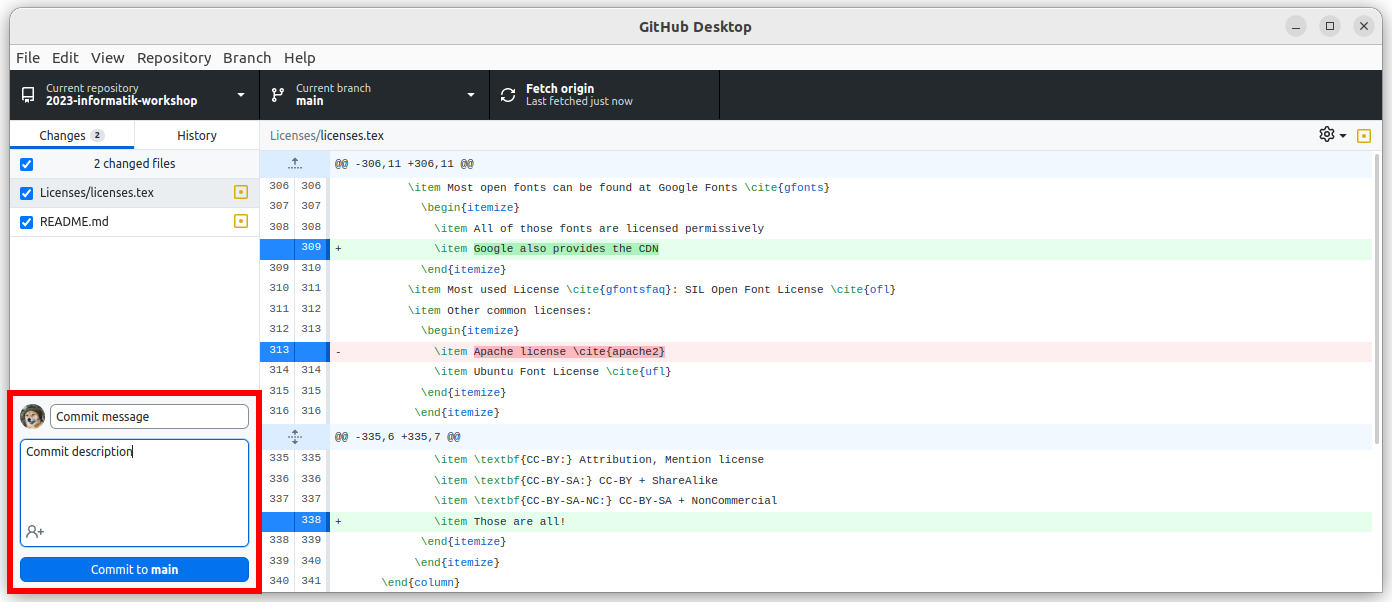
\includegraphics[height=0.75\textheight]{./assets/GH_02.png}
    \end{center}
  \end{frame}

  \begin{frame}{Pushing a Commit}
    \begin{center}
      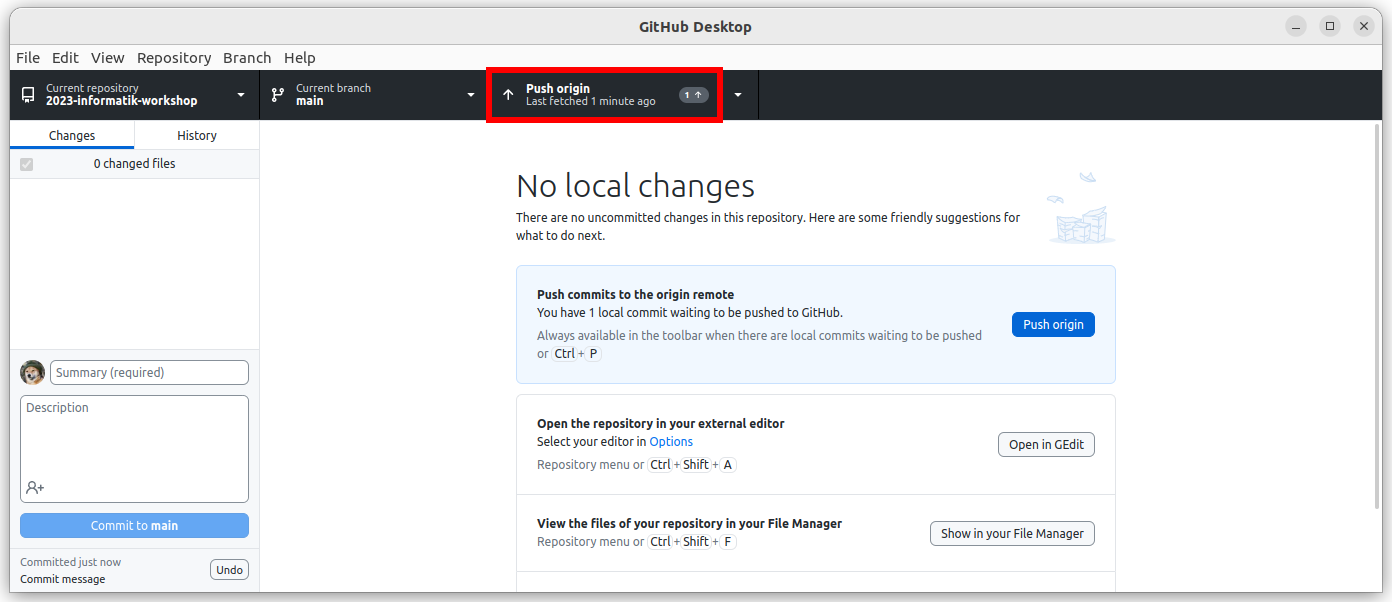
\includegraphics[height=0.75\textheight]{./assets/GH_03.png}
    \end{center}
  \end{frame}

	\section{Advanced}

	\begin{frame}{Problem: Merge Conflicts}
		\begin{itemize}
			\item Alice and Bob pull a project and work on it
      \item Alice changes \texttt{src/foo.c}
      \item Alice commits and pushes her update
      \item Bob changes \texttt{src/foo.c}
      \item Bob also commits and pushes his update
      \item But Bob's version doesn't have Alice's update!
		\end{itemize}
	\end{frame}

  \begin{frame}{Solution: Branching}
    \begin{itemize}
      \item Everybody uses their own \textbf{branch}
        \begin{itemize}
          \item Often around a \emph{feature}
        \end{itemize}
      \item Everybody can work without problems on their own
      \item Branches then can get \textbf{merged} when done
      \item Extreme example: Linux Kernel 66-way merge
    \end{itemize}
    \begin{center}
      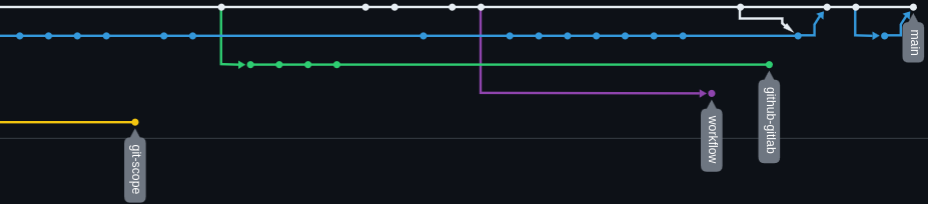
\includegraphics[width=0.8\textwidth]{./assets/guitarhero.png}
    \end{center}
  \end{frame}

  \begin{frame}{Advanced Features}
    \begin{columns}
      \begin{column}{0.5\textwidth}
        \begin{block}{Gitignore}
          \begin{itemize}
            \item Often, temporary files are generated
              \begin{itemize}
                \item log files
                \item \texttt{node\_modules}
                \item \texttt{.DS\_Store}, \dots
              \end{itemize}
            \item A \textbf{\texttt{.gitignore}} can list files to ignore by git
            \item Github provides templates for many languages!
              \begin{itemize}
                \item \href{https://github.com/github/gitignore}{\url{https://github.com/github/gitignore}}
              \end{itemize}
          \end{itemize}
        \end{block}
      \end{column}
      \begin{column}{0.5\textwidth}
        \begin{block}{git blame}
          \begin{itemize}
            \item Found a bug? Find out who did it.
            \item Maps each line to
              \begin{itemize}
                \item The commit it was added
                \item The author
              \end{itemize}
            \item Support for most text editors!
          \end{itemize}
        \end{block}
      \end{column}
    \end{columns}
  \end{frame}

  \begin{frame}{Advanced Features: \texttt{git bisect}}
    \begin{figure}
      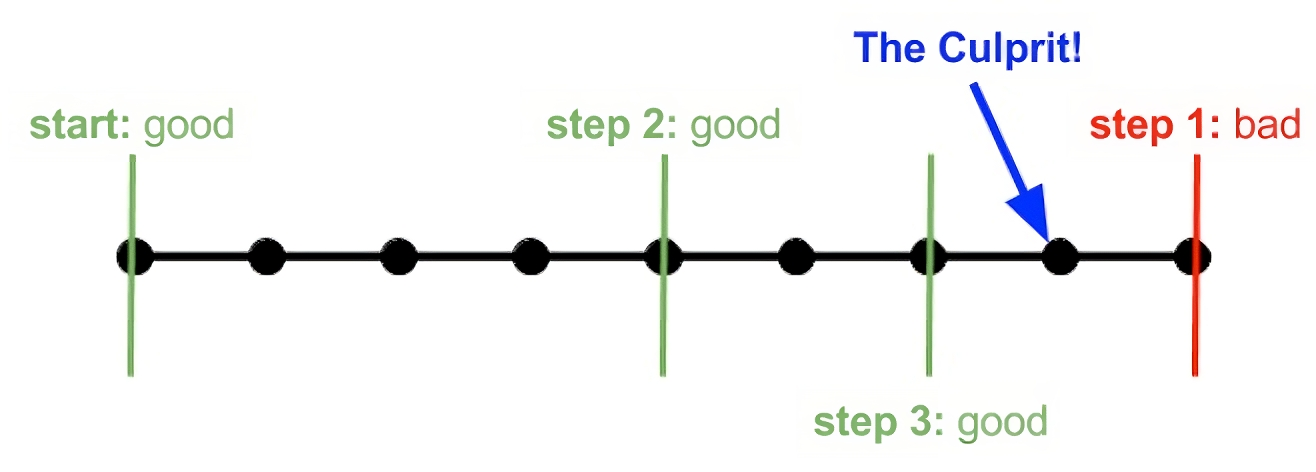
\includegraphics[width=\textwidth]{./assets/bisect.png}
      \caption{An example \texttt{bisect} \cite{bisect}}
    \end{figure}
  \end{frame}



	\section{Conclusion}

	\begin{frame}{Conclusion}
    \begin{block}{Summary}
      \begin{itemize}
        \item Git is a useful tool for code
        \item Starting a repo: \texttt{init} and \texttt{clone}
        \item Creating an update: \texttt{add}, \texttt{rm}, \texttt{commit}
        \item Updates: \texttt{push} and \texttt{pull}
        \item Branches and merges for collaboration
      \end{itemize}
    \end{block}
    \begin{block}{For many common problems:}
      \begin{center}
        \LARGE
        \href{https://ohshitgit.com/}{\url{https://ohshitgit.com/}}
      \end{center}
    \end{block}
		\label{pg:lastpage} % Label on last frame to get the page number for footer
	\end{frame}

	\begin{frame}{References}
		% References slide in appendix
		\renewcommand*{\bibfont}{\normalfont\scriptsize}
		\printbibliography[heading=none]
	\end{frame}

  \begin{frame}{Acknowledgements}
    \begin{itemize}
      \item Icons provided by \texttt{font-awesome} under the OFL license
    \end{itemize}
  \end{frame}

\end{document}
